\documentclass{beamer}

% Configuración para mostrar números en la tabla de contenidos
\setbeamertemplate{section in toc}[sections numbered]
\usetheme{Frankfurt}
\usepackage{graphicx}
\renewcommand{\normalsize}{\fontsize{7}{5}\selectfont} 

\title{Automatización del proceso de evaluación en exámenes de opción múltiple, un enfoque para optimizar la calificación y el registro de notas}
\author{Michael Santiago Jiménez Caballero}
\date{\today}


\begin{document} %_____________________________________**__________________________________

\frame{\titlepage}
\begin{frame}{Contenido}
    \tableofcontents
\end{frame}

\section{Resumen}
\begin{frame}{Resumen}
    En el presente documento se muestra el desarrollo de una aplicación web que automatiza la  calificación de exámenes de
    opción múltiple mediante redes neuronales convolucionales y  algoritmos de 
    reconocimiento óptico de caracteres. La implementación incluye una aplicación
    web y logra un 97\% de precisión, optimizando el proceso de evaluación y los recursos docentes.
\end{frame}

\section{Introducción}
\begin{frame}{Introducción}
    Se resalta la necesidad de automatizar la calificación de exámenes de opción múltiple en Colombia para reducir 
    la carga de los docentes y mejorar el enfoque en la enseñanza. Las limitaciones tecnológicas y el predominio 
    de métodos tradicionales, como el examen ICFES, refuerzan esta necesidad. Se propone un sistema de 
    calificación automática basado en OCR y dispositivos sencillos, como smartphones, para agilizar el 
    proceso y optimizar el tiempo dedicado a actividades pedagógicas.    
\end{frame}

\section{Problema}
\begin{frame}{Problema}
    Este proyecto destaca la importancia de automatizar la calificación en la educación básica, ofreciendo 
    una solución para optimizar el trabajo de los docentes en la evaluación de pruebas. Actualmente, 
    la calificación manual consume recursos significativos, limitando el enfoque en el aprendizaje. 
    La automatización no solo reduce este trabajo, también genera estadísticas descriptivas clave 
    sobre el desempeño estudiantil, facilitando decisiones pedagógicas más informadas, incluso en
     contextos con acceso tecnológico limitado.
\end{frame}

\section{Justificación}
\begin{frame}{Justficación}
    \begin{itemize}
        \item Se  plantea que el desarrollo de una aplicación que automatice la calificación de exámenes de selección múltiple, utilizando visión artificial.  puede permitir que el sistema obtenga una alta precisión, optimizando el trabajo docente y permitiendo el uso de recursos accesibles como smartphones. 
        \item Además, de agilizar la calificación, el proyecto promueve un equilibrio entre las tareas administrativas y pedagógicas, liberando recursos para mejorar la calidad del aprendizaje. Esta innovación responde a los desafíos actuales en la educación básica colombiana, destacando el impacto positivo de la automatización en el proceso educativo
    \end{itemize}
\end{frame}

\section{Objetivo General}
\begin{frame}{Objetivo General}
    \begin{itemize}
        \item Desarrollar un modelo de visión artificial para automatizar la calificación de exámenes de selección múltiple mediante algoritmos de reconocimiento óptico de caracteres, con el fin de reducir la carga laboral de los docentes.
    \end{itemize}
\end{frame}

\section{Objetivos Específicos}
\begin{frame}{Objetivos Específicos}
    \begin{itemize}
        \item Realizar funciones de preprocesamiento de las imágenes para la limpieza de estas.
        \item Implementar un algoritmo de Reconocimiento Óptico de Caracteres (OCR) para encontrar patrones en las imágenes, permitiendo la extracción automática de las respuestas seleccionadas por los estudiantes.
        \item Realizar un modelo que utilice redes neuronales convolucionales para la clasificación de múltiples clases.
        \item Desarrollar funciones vinculen el algoritmo de OCR con el modelo y permita reconocer como las opciones seleccionadas por cada estudiante, y las organice para su evaluación.
        \item Realizar pruebas exhaustivas del algoritmo OCR en diferentes tipos de hojas de respuestas, garantizando una precisión superior al 90\% en la detección de las respuestas.
        \item Desplegar los algoritmos en una aplicación web
    \end{itemize}
\end{frame}

\section{Antecedentes}
\begin{frame}{Antecedentes}
    \textbf{Sistema de Puntuación Automatizado para Exámenes de Opción Múltiple con Retroalimentación Rápida}
    \begin{itemize}
        \item Este proyecto se basa en el trabajo de Chai \& Alomran (2018), quienes utilizaron procesamiento de imágenes y OCR para automatizar la calificación de exámenes de opción múltiple.
        \item Su tecnología identifica respuestas manuscritas sin necesidad de formularios costosos ni equipos especializados.
        \item Mediante técnicas avanzadas de OCR, el sistema procesa hojas escaneadas, reconoce códigos de identificación y detecta las respuestas seleccionadas con alta precisión.
        \item Este modelo resalta que la automatización de la puntuación es eficiente, accesible y representa un avance importante en la mejora de los procesos educativos.
    \end{itemize}
\end{frame}

\begin{frame}{Antecedentes}
    \textbf{Android Based Automated Scoring of Multiple-Choice Test}
    \begin{itemize}
        \item Este proyecto propone una solución accesible y económica para automatizar la calificación de exámenes de opción múltiple, utilizando tecnologías como OCR y procesamiento de imágenes.
        \item Se emplean teléfonos inteligentes Android para reemplazar los lectores ópticos tradicionales, mejorando la accesibilidad en contextos con recursos limitados.
        \item El sistema detecta marcas de "X" en hojas de respuestas y alcanza un reconocimiento del 90\%, optimizando la evaluación educativa y reduciendo costos.
        \item Este enfoque es práctico y eficiente, adaptado a las necesidades actuales del ámbito educativo.
    \end{itemize}
\end{frame}



%------------------------------------------_____________________________________**__________________________________----------------------------------------------------------------


\section{Marco Teórico}
\begin{frame}{Marco Teórico}
    Los algoritmos de OCR permiten extraer información importante de las imágenes a través de diferentes parámetros, una vez se establecen es posible la recolección de información, la cual, se puede utilizar en un modelo de redes neuronales convolucionales (CNN), que se encargan de de claisificar de acuerdo con los diferentes mapas de características,
    pasando por diferentes procesos como la construcción del modelo utilizando CNN, construcción del algoritmo de reconocimiento óptico de caracteres
\end{frame}


\begin{frame}{Redes neuronales convolucionales CNN}
    \textbf{Definición}
    \[
    \]
    Las redes neuronales convolucionales (CNN), también conocidas como ConvNets, son una arquitectura especializada dentro del campo de las redes neuronales profundas. Están diseñadas específicamente para el procesamiento de datos de imágenes, siendo altamente efectivas en tareas como el reconocimiento de patrones y la clasificación de objetos. Su arquitectura está fundamentada en la operación matemática de la convolución, un proceso esencial en el análisis de señales que permite extraer características significativas de las imágenes procesadas.

\end{frame}


\subsection{Convolución}
\begin{frame}{Convolución}
    La convolución transforma datos de entrada, como imágenes, utilizando filtros llamados "Kernels" que extraen características. Matemáticamente, el resultado de la convolución se expresa como:
    \[
        S(i,j) = \sum\sum I(i + m, j + n) \cdot K(m, n)
    \]
    El Kernel recorre la imagen realizando un producto punto entre la imagen y el filtro, generando un "mapa de características". Este proceso consume muchos recursos, por lo que se recomienda usar capas de Pooling para optimizar el entrenamiento (Seiler \& Fergus, 2014).
    \begin{figure}
        \centering
        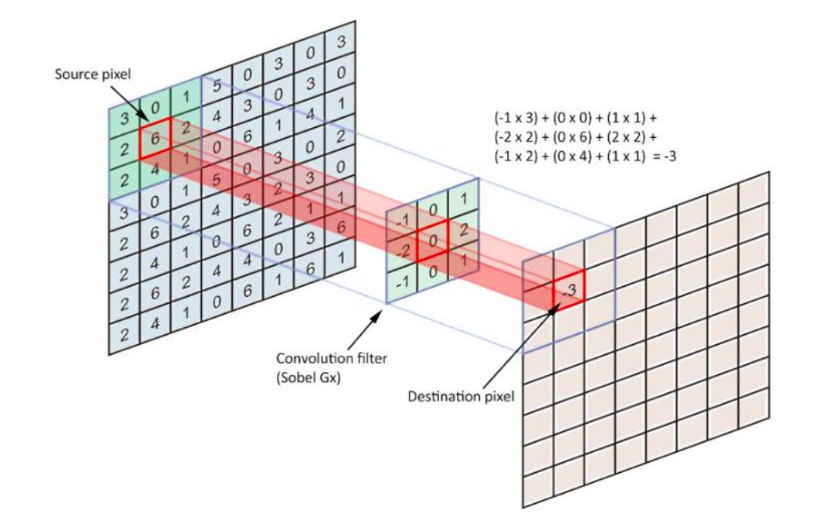
\includegraphics[width=0.5\textwidth]{/home/lic-jimenez/Documents/Tesis-Final/Slides/conv_1.png}
        
    \end{figure}
\end{frame}



\subsection{Pooling}
\begin{frame}{Pooling}
    \begin{itemize}
        \item \textbf{Función Principal} \[\] Las capas de pooling están diseñadas para reducir la dimensionalidad de los datos procesados por el Kernel. Este proceso disminuye el tamaño de la matriz de salida, reteniendo únicamente las características más relevantes y eliminando elementos no esenciales, como el ruido.
        \item \textbf{Max Pooling} \[\] Es el tipo más común de capa de pooling y opera de manera similar al Kernel.
        Utiliza matrices pequeñas, típicamente de tamaños 2*2 o 3*3, para seleccionar los valores de píxeles con mayor intensidad dentro de la escala de grises.
        Los valores con menor intensidad son descartados, lo que permite preservar información clave mientras se reduce significativamente la dimensionalidad de los mapas de características.
    \end{itemize}

    \begin{figure}
        \centering
        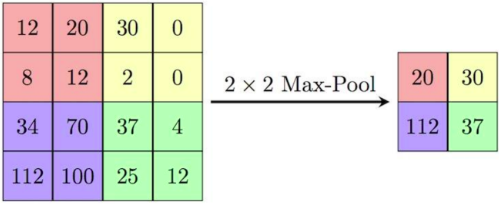
\includegraphics[width=0.5\textwidth]{/home/lic-jimenez/Documents/Tesis-Final/Slides/pool_1.png}
    \end{figure}
\end{frame}


\subsection{ReLU}
\begin{frame}{ReLU}
    Es frecuentemente utilizada después de las capas de pooling, ya que en este punto los objetos están suficientemente caracterizados con dimensiones reducidas. 
    \[ f(x) = max (0, x) \]
    Su funcionamiento es sencillo: evalúa cada elemento de la matriz de salida, reemplazando con 0 los valores menores o iguales a cero y conservando los valores positivos sin alteraciones. Esto permite que los valores positivos se transmitan intactos a la siguiente capa, mientras que los negativos se eliminan.    
    \begin{figure}
        \centering
        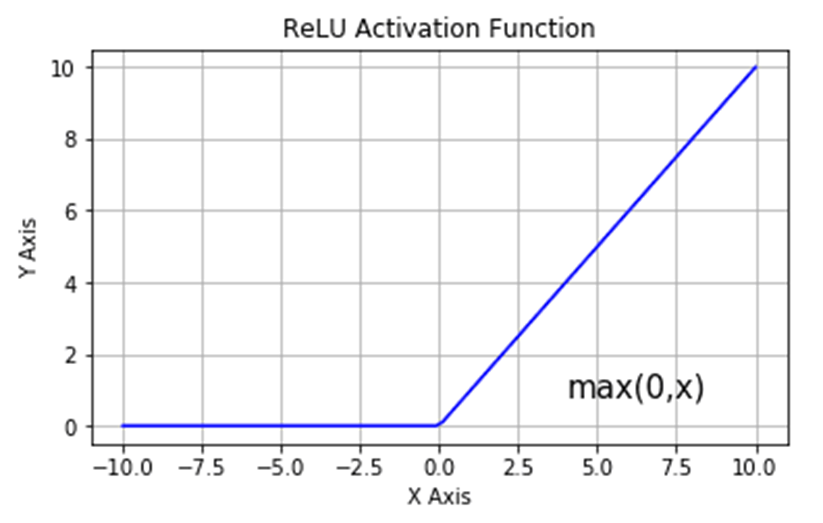
\includegraphics[width=0.5\textwidth]{/home/lic-jimenez/Documents/Tesis-Final/Slides/ReLU_1.png}
    \end{figure}
\end{frame}


\subsection{Capas Flatten}
\begin{frame}{Capas Flatten}
Las capas Flatten se utilizan para convertir mapas de características multidimensionales en un vector unidimensional, esencial para conectar dichas características con las capas completamente conectadas. Por ejemplo, en imágenes en escala de grises, el mapa tiene dos dimensiones principales (altura y ancho), con una tercera dimensión que representa los niveles de intensidad (tonalidades). La capa Flatten toma este tensor tridimensional y lo transforma en un vector, cuya longitud es el producto de las dimensiones originales.
    \begin{figure}
        \centering
        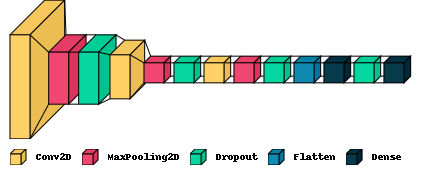
\includegraphics[width=0.5\textwidth]{/home/lic-jimenez/Documents/Tesis-Final/Slides/flatten.png}
    \end{figure}
\end{frame}


\subsection{Capas Dense}
\begin{frame}{Capas Dense}
    El vector unidimensional proveniente de la capa Flatten contiene información representativa de las características extraídas, donde cada elemento refleja patrones relevantes asociados a las clases procesadas. A través de la conexión completa de las neuronas, las capas Dense consolidan esta información y determinan cómo se relacionan las clases entre sí, ayudando al modelo a identificar con precisión a qué clase pertenece cada elemento evaluado.
\end{frame}



\subsection{Función Softmax}
\begin{frame}{Función Softmax}  
    La función Softmax es esencial en problemas de clasificación multiclase, como los abordados en este proyecto, donde se trabajó con 36 clases. Su uso permite transformar un vector unidimensional (proveniente de la capa Flatten) en probabilidades asociadas a cada clase, facilitando la clasificación. La función se define como:
    \[
   softmax(z_i) = \frac{e^{z_i}}{\sum_j e^{z_j}}
    \]
    El valor resultante oscila entre 0 y 1, representando la probabilidad de que un elemento pertenezca a una clase específica. Valores cercanos a 0 indican baja probabilidad de pertenencia, mientras que aquellos próximos a 1 reflejan una alta probabilidad. De este modo, Softmax permite asociar cada clase con un mapa de características específico, facilitando la clasificación final basada en las probabilidades calculadas.
    
\end{frame}


\subsection{Estructura de la red}
\begin{frame}{Estructura de la red}
    \begin{figure}
        \centering
        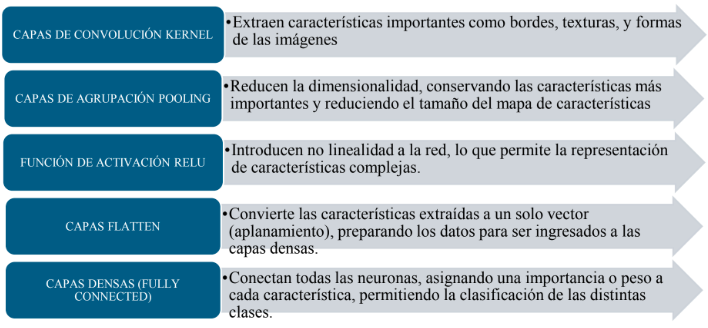
\includegraphics[width=1\textwidth]{/home/lic-jimenez/Documents/Tesis-Final/Slides/resume_1.png}
    \end{figure}
\end{frame}


\subsection{Sistema de calificación}
\begin{frame}{Sistema de calificación}
    \begin{itemize}
        \item \textbf{Accuracy}: También conocido como precisión, es la proporción de las diferentes clases identificadas correcta o incorrectamente (usualmente se utiliza de forma aprobatoria), entre el total de imágenes predichas, obteniendo un resultado entre 0 y 1, donde los valores cercanos a 1 muestran que el modelo reconoce satisfactoriamente las imágenes, por otra parte, cuando se aproxima a 0 da razón de una mala identificación.    
        \[
        Accuracy = \frac{True predictions}{Total predictions}
        \]
        \item \textbf{Recall}: Está dado por aquellas predicciones realizadas por el modelo en las imágenes tanto de entrenamiento como de validación, en las que evalúa los verdaderos positivos entre la suma de los verdaderos positivos y los falsos negativos
        \[
        Recall = \frac{TP_i}{TP_i+FN_i}
        \]
        \item \textbf{F1-score}: Se puede considerar el f1-score como el punto medio entre el Accuracy y Recall, dado que evalúa tanto los verdaderos positivos, falsos negativos y los correctamente identificados
        \[
        F1 = \frac{2*Accuracy*Recall}{Accuracy+Recall}
        \]
    \end{itemize}
\end{frame}

\subsection{Reconocimiento Óptico de Caracteres}
\begin{frame}{Reconocimiento Óptico de Caracteres}
    \begin{itemize}
        \item El reconocimiento óptico de caracteres (OCR) basado en redes neuronales convolucionales (CNN) es una técnica avanzada que permite convertir texto en imágenes a texto digital. Según Doermann y Tombre (2014), las CNN son ideales para esta tarea debido a su capacidad de extraer características jerárquicas y patrones a distintos niveles de abstracción, haciéndolas altamente efectivas en tareas de visión por computadora.
        \item No obstante, durante este proyecto, no se logró implementar satisfactoriamente tecnologías conocidas de OCR debido a limitaciones relacionadas con la variabilidad en letras, fuentes, estructuras y lenguajes. Drobac y Lindén (2020) señalan que estos desafíos han existido desde las primeras etapas del desarrollo de algoritmos OCR.
        \item Pese a estas limitaciones, las CNN representan una herramienta robusta y adaptable, capaz de enfrentarse a escenarios complejos y variables en el reconocimiento de caracteres.
        
    \end{itemize}
\end{frame}


\section{Metodología}
\begin{frame}{Metodología}
    \begin{itemize}
        \item Considerando que el punto central de este trabajo es el desarrollo e implementación de un sistema de
        automatización para la calificación de exámenes de opción múltiple, se determina que el enfoque
        metodológico para la investigación será cuantitativo, usando un diseño transeccional predictivo.
    \end{itemize}    
\end{frame}


\subsection{Vinculación del OCR y el modelo de CNN}
\begin{frame}{Vinculación del OCR y el modelo de CNN}
    Se decidió construir un algoritmo de OCR especializado en la detección de caracteres en exámenes de opción múltiple y el proceso está basado en redes neuronales convolucionales.

    \begin{figure}
        \centering
        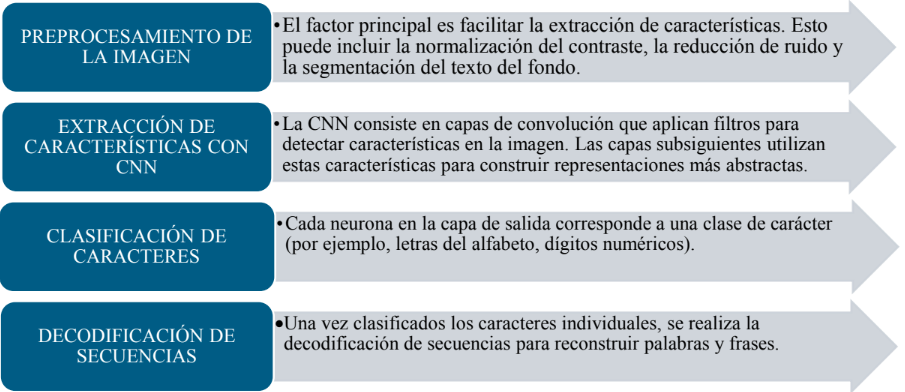
\includegraphics[width=1\textwidth]{/home/lic-jimenez/Documents/Tesis-Final/Slides/resume_2.png}
    \end{figure}
\end{frame}



\subsection{Formato de preguntas}
\begin{frame}{Formato de preguntas}
    La forma en la que el modelo recibe tanto el número de preguntas como su respectiva respuesta es utilizando números y letras. Se debe considerar que la primera columna referente a la pregunta y respuesta no se tiene en cuenta a la hora de hacer la evaluación. A partir de la segunda columna se encuentran en la primera fila los números correspondientes a la pregunta y en la segunda fila las letras respectivas a las respuestas.  
    \begin{figure}
        \centering
        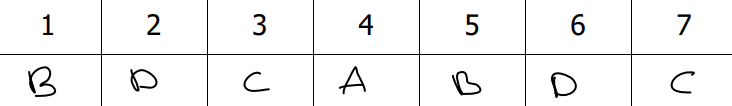
\includegraphics[width=1\textwidth]{/home/lic-jimenez/Documents/Tesis-Final/images_test/img_001.png}
    \end{figure}
\end{frame}


\subsection{Conjunto de datos}
\begin{frame}{Conjunto de datos}
    Una vez establecido el formato y limitaciones de este, se determinó que se usará MNIST para realizar el entrenamiento del modelo predictivo. Las razones por las que se eligió son las siguientes: MNIST NUMBERS que contiene 70.000 imágenes, divididas en 60.000 de entrenamiento y 10.000 de validación, donde cada número tiene entre 7.000 y 8.000 imágenes. Por otra parte, para las letras se utilizó el conjunto de datos proporcionado por (IA Expert Academy, s.f.), en el que se contiene 372.450 registros fotográficos de letras escritas a mano, en general de cada dígito hay entre cinco mil y diez mil imágenes. 
    \begin{figure}
        \centering
        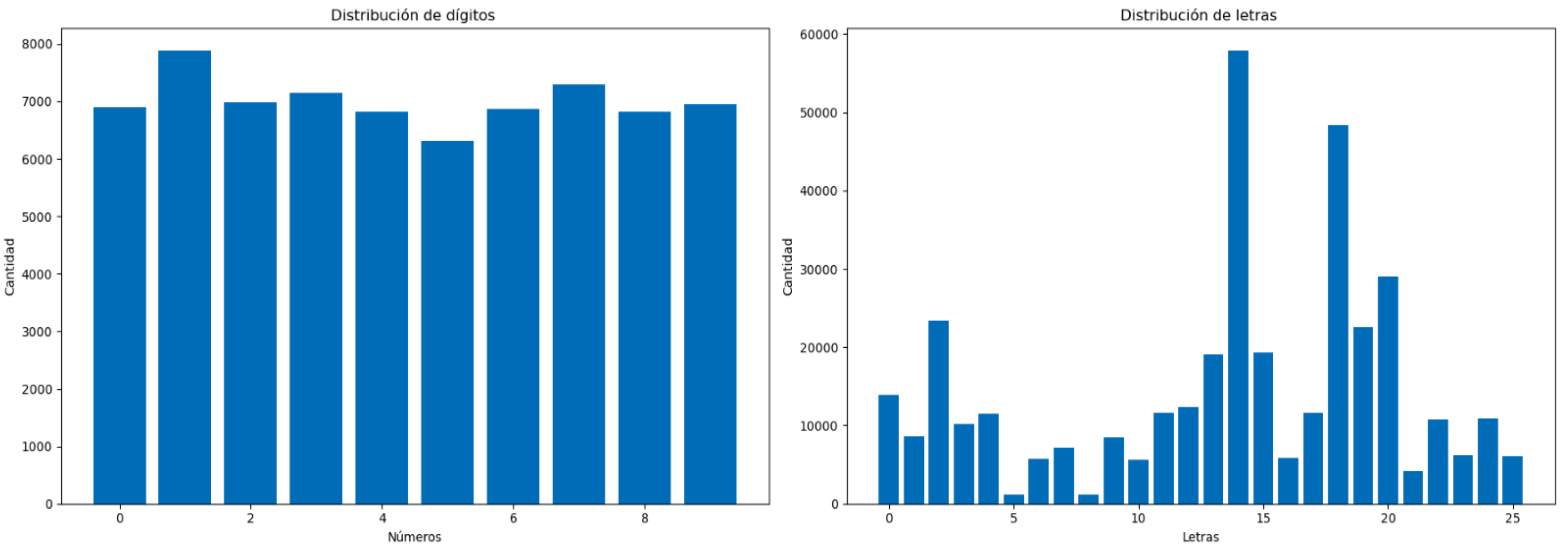
\includegraphics[width=1\textwidth]{/home/lic-jimenez/Documents/Tesis-Final/Slides/dataset.png}
    \end{figure}
\end{frame}


\subsection{Estructura CNN}
\begin{frame}{Estructura CNN}
    \begin{figure}
        \centering
        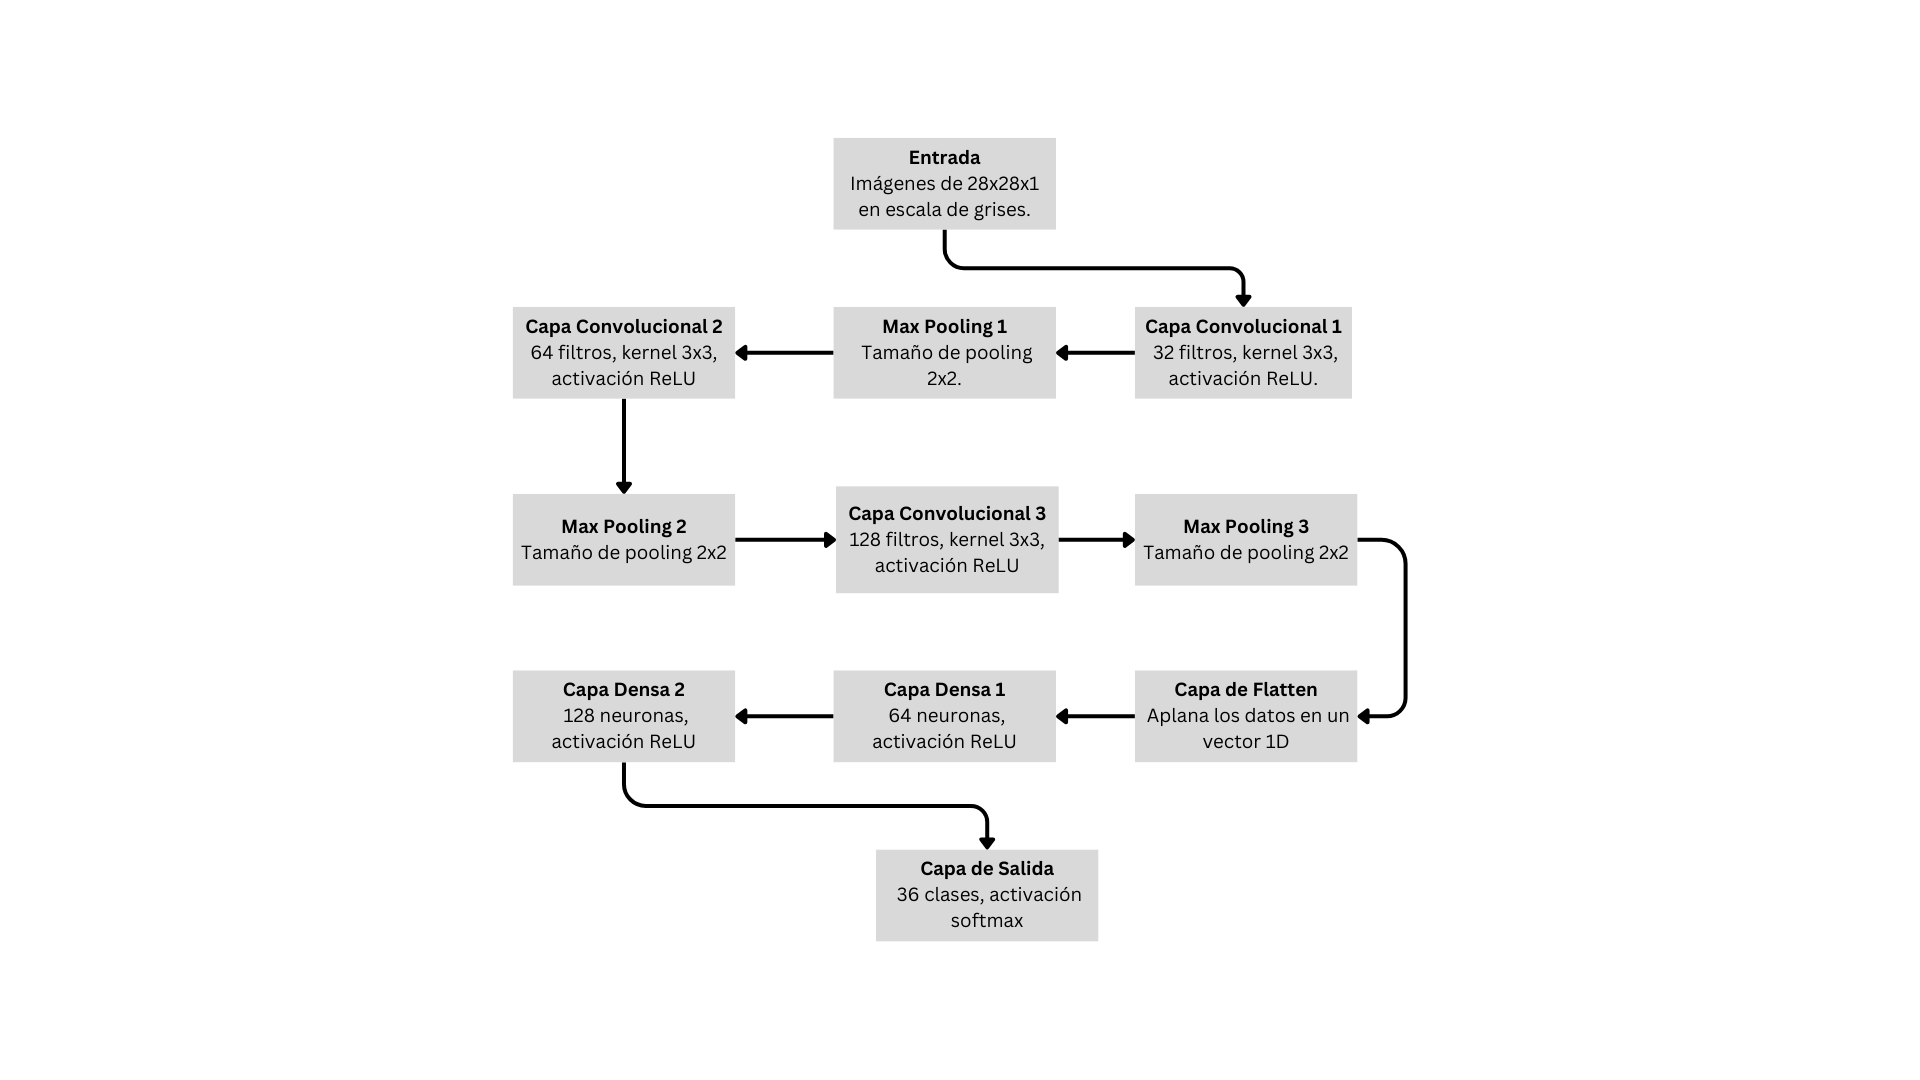
\includegraphics[width=1\textwidth]{/home/lic-jimenez/Documents/Tesis-Final/Slides/estructura_cnn.png}
    \end{figure}
\end{frame}



\subsection{Estructuración de OCR y CNN}
\begin{frame}{Estructuración de OCR y CNN}
    \begin{figure}
        \centering
        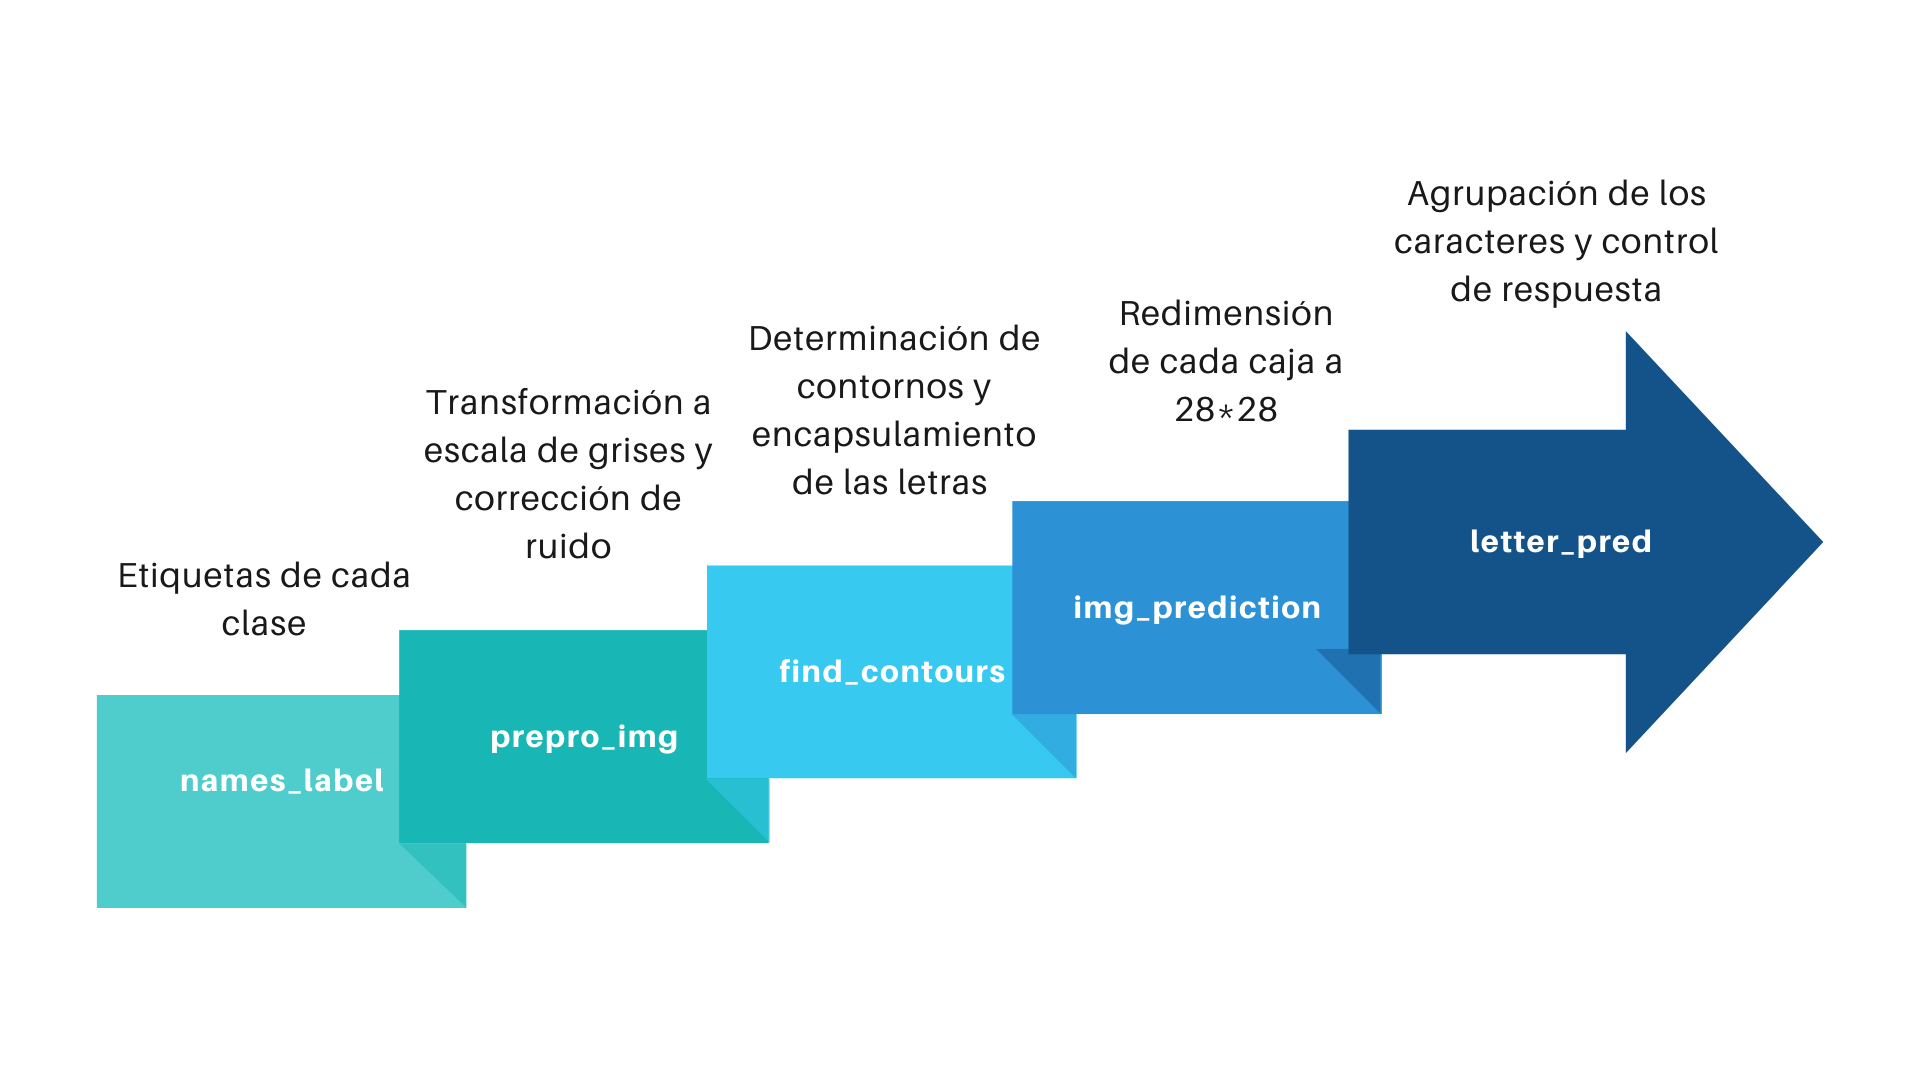
\includegraphics[width=1\textwidth]{/home/lic-jimenez/Documents/Tesis-Final/Slides/estructura_ocr.png}
    \end{figure}
\end{frame}



\subsection{Estructura del aplicativo web}
\begin{frame}{Estructura del aplicativo web}
    \begin{figure}
        \centering
        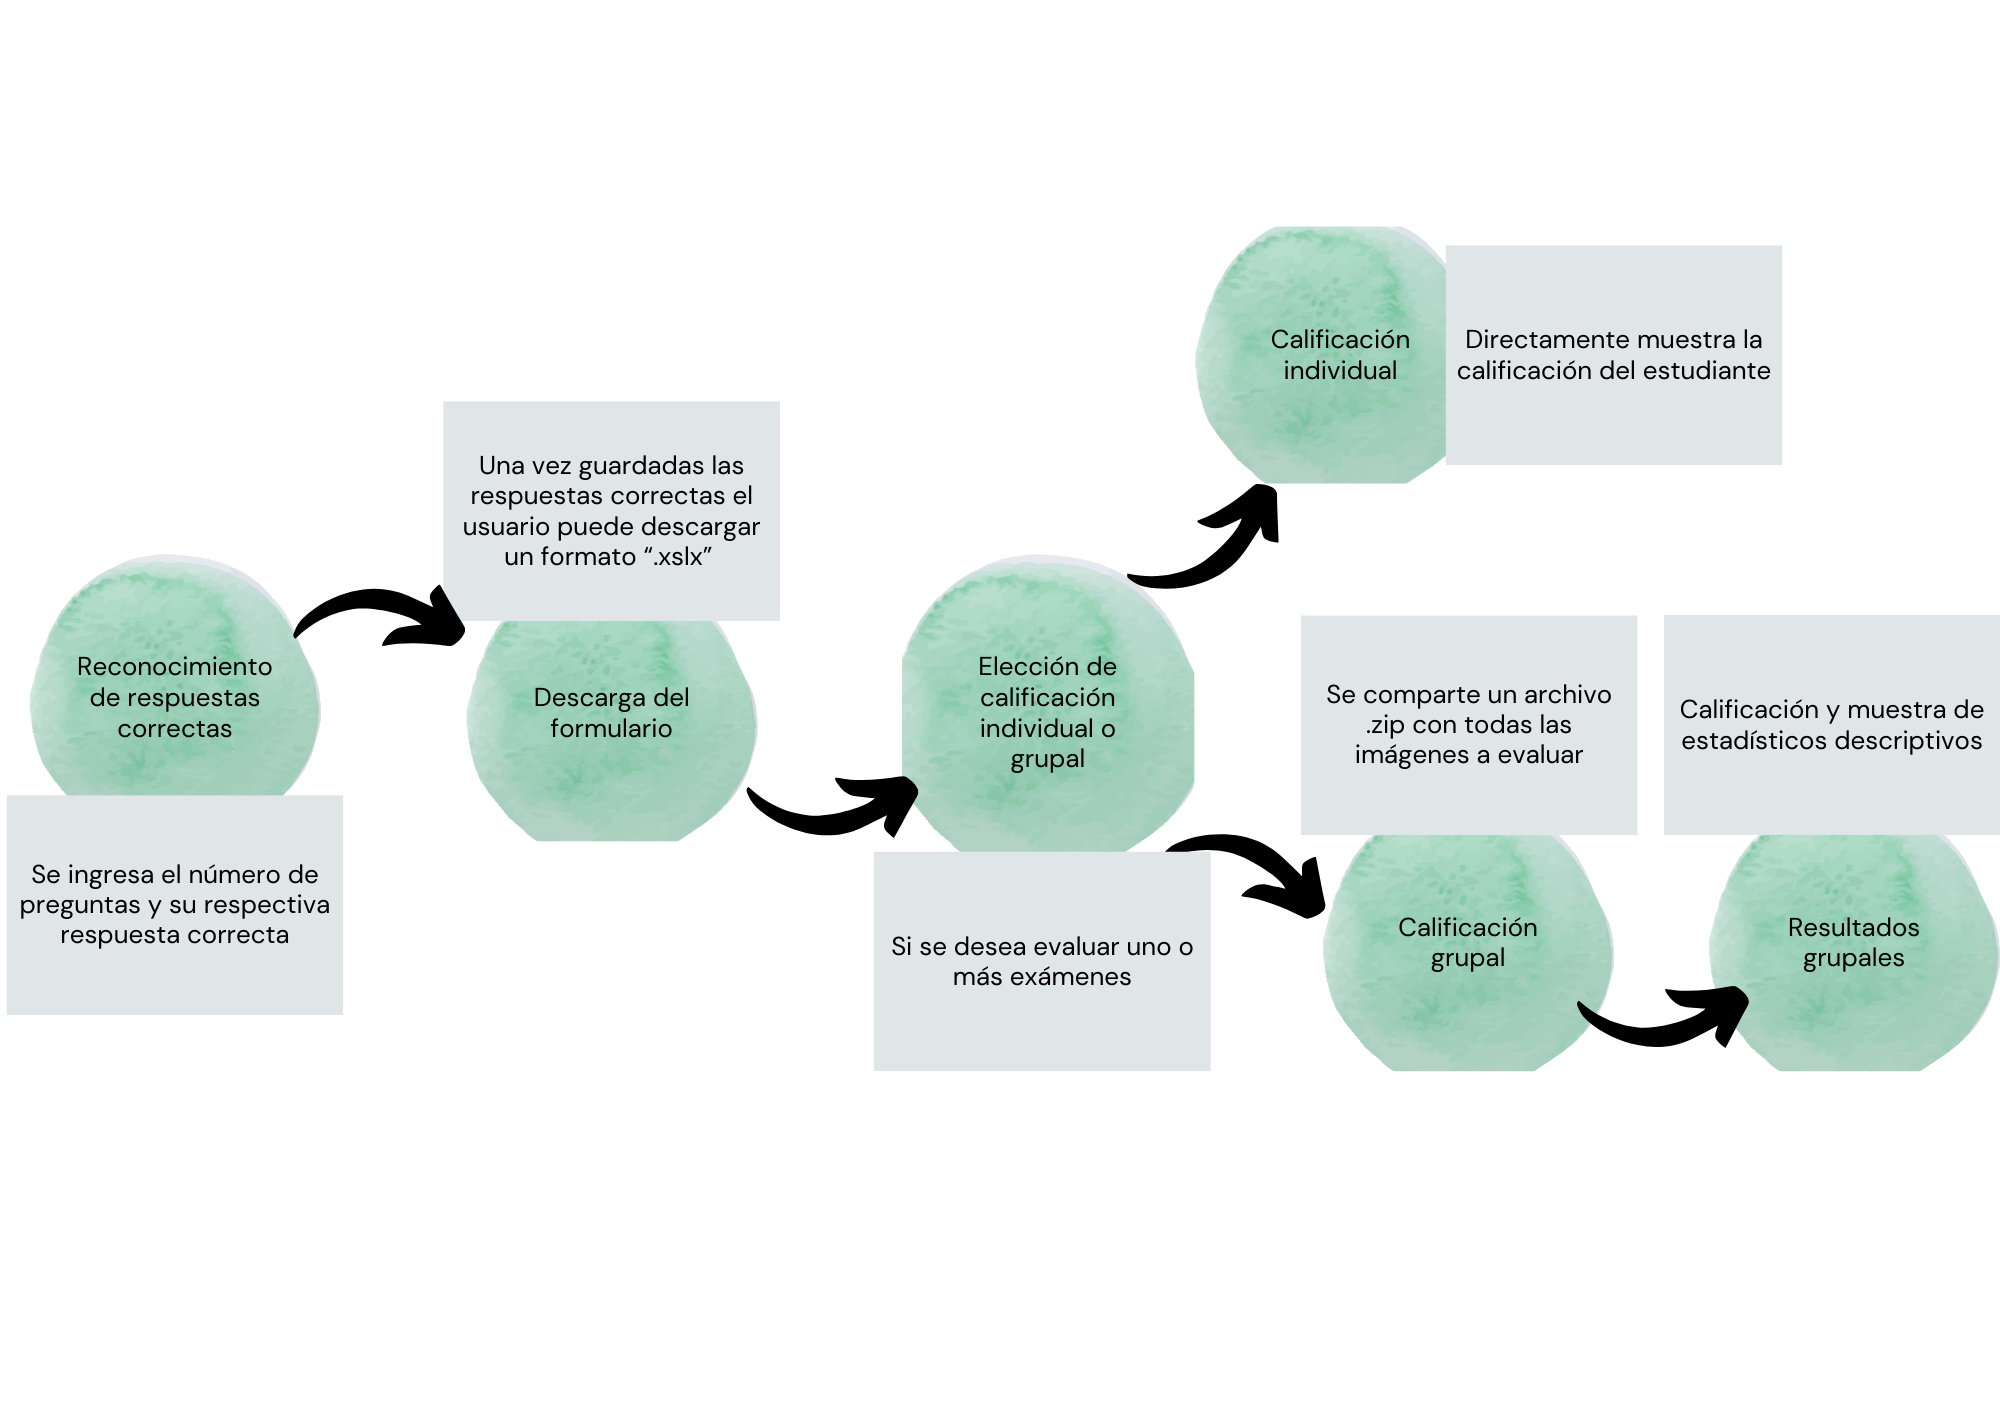
\includegraphics[width=1\textwidth]{/home/lic-jimenez/Documents/Tesis-Final/Slides/estructura_web.png}
    \end{figure}
    
\end{frame}


\section{Conclusiones}
\begin{frame}{Conclusiones}
    A continuación se mostrarán algunas de las conclusiones a las que se llegaron
    \begin{itemize}
        \item Desempeño del modelo
        \item Impacto en la educación 
        \item Limitaciones del sistema 
        \item Recomendaciones para el uso 
        \item Perspectivas futuras
    \end{itemize}
\end{frame}


\subsection{Desempeño del modelo}
\begin{frame}{Desempeño del modelo}
    \begin{itemize}
        \item Se desarrolló e implementó un modelo basado en redes neuronales convolucionales, logrando métricas sobresalientes con una precisión (accuracy) de 0.95, un recall de 0.95 y un f1-score de 0.96, lo que asegura una clasificación eficiente de las clases evaluadas.
        \item Al integrarse con un algoritmo OCR para la calificación de exámenes de opción múltiple, el sistema alcanzó una precisión de 0.97 en la clasificación de imágenes completas y una precisión general de 0.99 en la detección de caracteres individuales.

    \end{itemize}
\end{frame}


\subsection{Impacto en la educación}
\begin{frame}{Impacto en la educación}
    \begin{itemize}
        \item SEste proyecto demuestra que es posible automatizar la calificación de exámenes con alta precisión, optimizando el trabajo docente y permitiendo que los recursos se destinen a actividades educativas más relevantes.
        \item La solución no solo facilita la evaluación eficiente, sino que también genera confianza en la implementación de tecnologías avanzadas en contextos educativos.
    \end{itemize}
\end{frame}



\subsection{Limitaciones del sistema}
\begin{frame}{Limitaciones del sistema}
    \begin{itemize}
    \item El modelo funciona de manera óptima para exámenes con hasta siete preguntas y opciones de respuesta de "A" a "F".
    \item Los números "0" y "5" presentan un rendimiento bajo debido a confusiones con las letras "O" y "S", respectivamente. Sin embargo, estas limitaciones no afectan significativamente el desempeño general del modelo.
    \item Todas las respuestas deben estar en letras mayúsculas y escritas claramente para garantizar una detección correcta. Los bordes de las letras no deben solaparse con los márgenes de las celdas.
    \end{itemize}
\end{frame}


\subsection{Recomendaciones para el uso}
\begin{frame}{Recomendaciones para el uso}
    \begin{itemize}
        \item Siguiendo las instrucciones establecidas sobre claridad y formato de las respuestas, el aplicativo garantiza una calificación precisa y confiable.
        \item Es fundamental mantener el diseño del examen dentro de los parámetros definidos para evitar errores en el proceso de evaluación.

    \end{itemize}
\end{frame}


\subsection{Perspectivas futuras}
\begin{frame}{Perspectivas futuras}
    \begin{itemize}
        \item Extender las funciones del algoritmo OCR para incluir la identificación del estudiante y vincular esta información con una base de datos que registre su desempeño académico.
        \item Desarrollar un sistema que permita calificar tanto exámenes de selección múltiple como preguntas abiertas mediante algoritmos avanzados de OCR.
        \item Mejorar el manejo de caracteres ambiguos (como "0" y "5") para aumentar la versatilidad y robustez del modelo.
    \end{itemize}
\end{frame}



\end{document}
